\section{Introduction}
\label{sec:intro}

The rapid evolution of Large Language Model (LLM) agents has sparked a large body of exciting research and industrial efforts in building agent memory, i.e., the data management system of the LLM agent that supports long-horizon stateful execution and personalized interaction~\cite{luo2026data,khan2026rag,liu2026supporting,singh2024personal,openai2026agents,microsoft2025copilot,google2025adk}. 

As shown in Figure~\ref{fig:intro}, existing agent memory systems span a diverse set of architectural designs. %\texttt{(1) RAG-based Memory System} (e.g., LangChain~\cite{langchain2026harness}) embeds past interactions or external documents into dense vectors and stores them in stateless vector databases (e.g., FAISS~\cite{johnson2019billion}) for top-$k$ similarity search. 
\textsf{(1) Stream-and-Reflection Memory System} (e.g., MemoryBank~\cite{memorybank}) maintains experiences as timestamped memory streams and periodically summarizes them into higher-level reflections that are written back into the stream; 
\textsf{(2) Hierarchical Tiered Memory System} (e.g., MemGPT~\cite{packer2023memgpt}) organizes memory into multiple levels with different capacities and access properties, separating core memory from archival storage with explicit movement (e.g., eviction and promotion) across tiers; 
\textsf{(3) Knowledge Graph Memory System} (e.g., $\text{Mem0}^g$~\cite{chhikara2025mem0}, Zep~\cite{rasmussen2025zep}) represents entities, relations, and their temporal evolution in structured forms (e.g., temporal knowledge graphs), often incorporating entity disambiguation and conflict resolution; \textsf{(4) Composite Hybrid Memory System} (e.g., A-MEM~\cite{xu2025amem}) routes schema-aware memory objects across multiple storage substrates, explicitly separating runtime state (e.g., KV caches) from long-term storage (e.g., vector, graph, keyword indexes), managed by dedicated maintenance modules. However, this rapid proliferation has also led to a highly fragmented landscape that lacks systematic evaluation from a data management perspective, raising a natural question: \textit{Are we ready for an agent-native memory system?}


% \begin{figure}[!t]
%     \centering
%     \vspace{1em}
%     \begin{subfigure}{0.5\textwidth}
%         % , trim={0em 1em 5em 0}, clip
%         \includegraphics*[width=\textwidth]{figures/intro_example_workflows_v6}
%         %\caption{Agent Memory vs. Database System.}
%         % \vspace{3pt}
%         % \label{fig:cpu-kp}  
%     \end{subfigure}
%     % \begin{subfigure}{0.45\textwidth}
%     %     \includegraphics*[width=\textwidth]{figures/intro_performance.pdf}
%     %     \caption{Agent Memory Performance}
%     %     % \vspace{3pt}
%     %     % \label{fig:cpu-kp}  
%     % \end{subfigure}
%      \vspace{-2em}
%     \caption{Typical Execution Workflows of Agent Memory.
%     %Execution Workflows of Agent Memory \zw{notice RAG might not fail into memory system within current context}.% (a) Context Window Memory (e.g., MEM1),  Performance of Different Agent Memory Methods \zw{(to be refined, (a) comparison of agent memory and database system, (b) trending of agent memory systems)}.  \textnormal{-- (a) RAG-Based External Memory (e.g., Mem0, LangChain), (b) OS-Inspired Tiered Memory (e.g., MemGPT), (c) Memory Stream + Reflection (e.g., MemoryBank), (d) Knowledge Graph Memory (e.g., Zep, Mem0g), (e) Composite Hybrid Memory (e.g., MemOS, A-MEM, MIRIX, SimpleMem, EverMemOS)
%     }
%     % \vspace{-.25em}
%     \label{fig:intro}
%     \vspace{-.5cm}
% \end{figure}


\begin{figure}[!t]
  \centering
  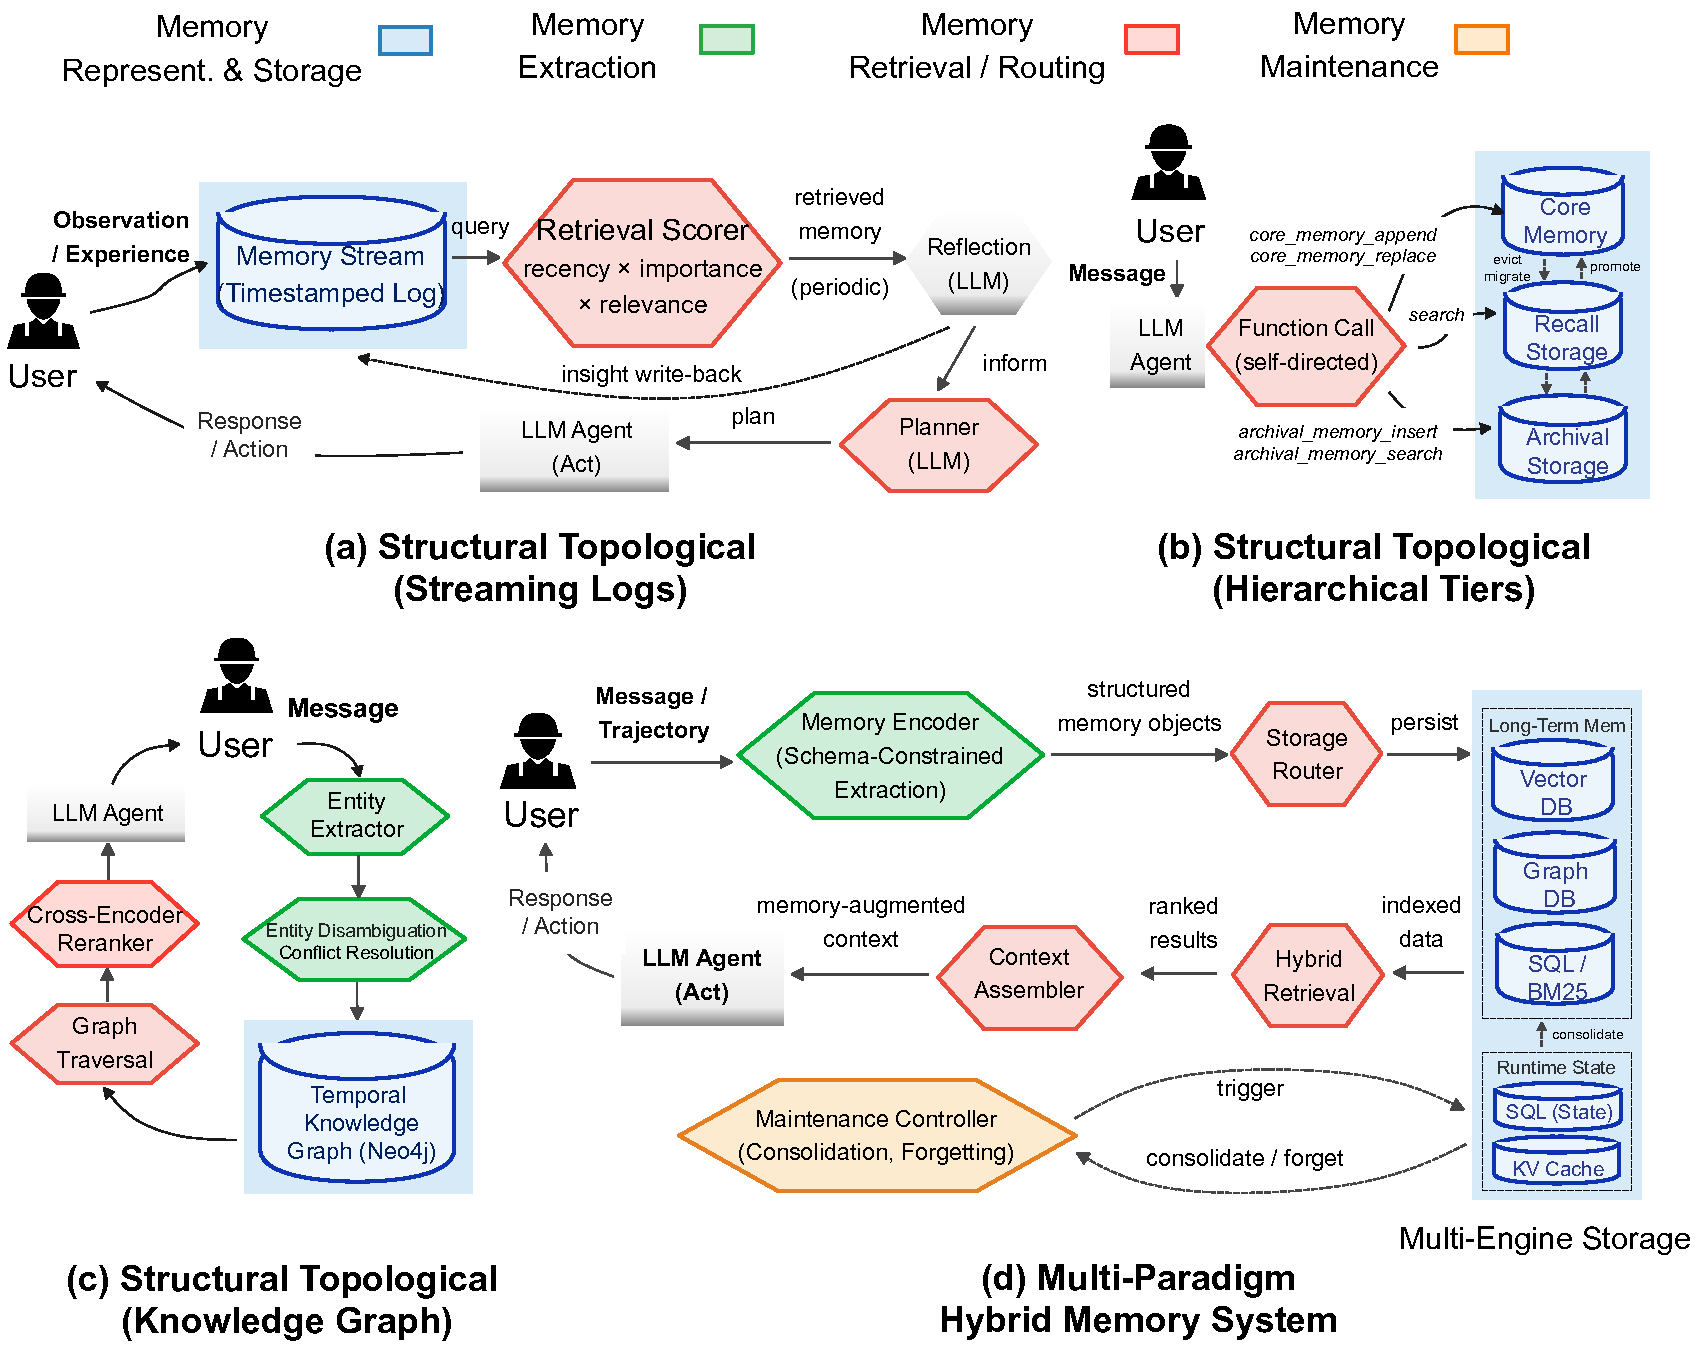
\includegraphics[width=\linewidth]{figures/intro_example_workflows_v6.pdf}
  \vspace{-.5cm}
  \caption{Typical Execution Workflows of Agent Memory.}
  \label{fig:intro}
  \vspace{-.5cm}
\end{figure}


In this paper, we revisit this question for agent memory. In particular, we focus on \textit{system-level memory} over textual, structured, and even parametric representations~\cite{chhikara2025mem0,packer2023memgpt,rasmussen2025zep,xu2025amem}, a fundamental infrastructure component for modern autonomous agents.
We focus on memory-centric systems, rather than task-specific agent frameworks where memory is an auxiliary module~\cite{claudecode, zhou2026dbcooker}.
It is the persistent data management system that maintains information beyond a single inference step (e.g., historical interactions, environmental observations, and intermediate tool executions) decoupled from the LLMs' parametric weights and volatile context windows. Agent frameworks rely on these external memory systems (e.g., Mem0~\cite{chhikara2025mem0}, Letta~\cite{packer2023memgpt}, Zep~\cite{rasmussen2025zep}, and A-MEM~\cite{xu2025amem}) to actively write, update, index, and route relevant context back into the reasoning loop. The capability of a long-horizon agent largely depends on the reliability and efficiency of this memory layer. An agent adopting a poorly designed memory architecture can suffer from factual contradictions, catastrophic forgetting, or unacceptable latencies during continuous execution~\cite{du2026memory,zheng2025lifelong}.

Recent benchmarks~\cite{maharana2024locomo,wu2024longmemeval,memoryagentbench2026,membench} have evaluated agent memory and shown that external memory can improve agent performance on tasks requiring factual recall and long-context understanding. However, these evaluations are largely rooted in natural language processing and have multiple limitations when treating agent memory as a data management system (see Section~\ref{sec:def}). 
First, they fail to evaluate many representative memory architectures (e.g., systems such as MemoChat, MemTree, and LightMem have not been included in prior evaluations) under unified workloads, making principled cross-system comparisons difficult. Efforts from the database community~\cite{wu2026memoryeab} limit their scope to a few chatbot-centric datasets (e.g., LoCoMo and LongMemEval only), neglecting complex agentic execution scenarios. 
Second, existing benchmarks predominantly rely on single-sided, end-to-end task success metrics (e.g., F1 and BLEU scores) rather than a comprehensive evaluation suite. They fail to explicitly isolate and measure multi-dimensional performance indicators such as evidence-level retrieval fidelity, dynamic update robustness under conflicting knowledge, and long-horizon stability. 
Third, they rarely measure key operational costs from a systems perspective, such as index construction time and query latency, which are critical for production deployments.
Last, they treat memory systems as monolithic black boxes rather than decomposing them into fundamental data management modules for isolated, fine-grained analysis.

We overcome these limitations and conduct comprehensive experiments and analyses from a data management perspective. The contributions are as follows.

\noindent
\textbf{(1) Technology Decomposition and Taxonomy (Section~\ref{sec:overview}).}
We decompose existing agent memory systems into four core components: (i) memory representation and storage, (ii) memory extraction, (iii) memory retrieval and routing, and (iv) memory maintenance. For each component, we further establish a structured taxonomy\footnote{\blue{\url{https://github.com/OpenDataBox/awesome-agent-memory}}} by categorizing existing approaches according to their underlying design principles, enabling principled comparisons.

\noindent
\textbf{(2) Overall End-to-End Performance Evaluation (Section~\ref{sec:overall}).}
We conduct end-to-end evaluations under a unified and fair testbed (e.g., {unified time-overhead traces})\footnote{\blue{\url{https://github.com/OpenDataBox/MemoryData}}} across five distinct benchmark workloads encompassing 11 datasets. Our study includes 12 representative memory systems, each embodying different combinations of representation, storage, routing, and maintenance strategies. We evaluate their performance from five perspectives: task effectiveness (RQ1), retrieval fidelity (RQ2), dynamic update robustness (RQ3), long-horizon stability (RQ4), and operational cost (RQ5).

\noindent
\textbf{(3) Fine-Grained Technical Component Evaluation (Section~\ref{sec:finegrained}).}
Leveraging our four-module framework, we conduct controlled and fine-grained experiments on representative strategies within each technique component. By systematically generating controlled variants that modify one module at a time, we quantify their performance trade-offs and assess their individual impacts on representation fidelity, routing precision, and update correctness.

\noindent
\textbf{(4) Insightful Findings.}
Based on our experimental results and in-depth analysis, we distill a set of insightful findings regarding the cost--performance trade-offs of agent memory systems:

\noindent
\ding{182} \textbf{Are Memory Systems Effective Across Different Agent Request Workloads?} No single memory architecture dominates all scenarios. Composite hybrid systems lead on conversational QA, while graph-based methods excel in single-hop factual recall but struggle with temporal reasoning. Moreover, effective memory systems remain robust across \llm backbone variants because they externalize evidence localization before answer generation.

\noindent
\ding{183} \textbf{How Accurately Do Memory Systems Retrieve Stored Evidence?} Explicit query planning and balanced hybrid search maximize contextual relevance. However, retrieval accuracy degrades significantly as the temporal distance between the evidence and the query increases, exposing limitations of similarity-based retrieval.

\noindent
\ding{184} \textbf{Are Memory Systems Robust Under Dynamic Updates?} Graph-based methods handle knowledge updates most reliably, whereas popular fact-extraction plugins and append-only stores struggle with targeted overwrites. Systems lacking lifecycle management return stale facts, leading to ``hallucinations of the past''.

\noindent
\ding{185} \textbf{Do Memory Systems Remain Stable Over Long Horizons?} Many append-only memory stores suffer from catastrophic degradation as evidence becomes more distant. For time-dependent queries, raw long-context retrieval still outperforms most memory-backed approaches, indicating that standard semantic consolidation often destroys crucial chronological cues.

\noindent
\ding{186} \textbf{What Are the Operational Costs of Agent Memory?} Highly structured systems incur orders-of-magnitude higher index construction time and query latency than lightweight stores, yet do not consistently deliver proportional accuracy gains.

\noindent
\ding{187} \textbf{When Do Individual Memory Components Go Wrong?} Each layer of abstraction (e.g., compression, summarization, and fact extraction) progressively discards information. Furthermore, fine-grained \llm-based extraction can yield modest precision gains but substantially degrade multi-hop reasoning. Finally, conservative memory consolidation serves as the best default maintenance strategy, whereas delayed flushing creates a deceptive trade-off between surface-level coverage and actual answerability.

% \noindent
% \textbf{(5) Usage Guidelines and Research Directions (Section~\ref{sec:conclusion}).}
% We summarize practical guidelines for selecting and configuring agent memory systems, and outline several promising research directions for the database community, including specialized storage engines, cost-based memory query optimizers, and multi-agent consistency models. We publish our code and datasets on GitHub\footnote{\url{https://anonymous.4open.science/r/MemoryData-08F6}} to facilitate future research.


\iffalse
\hi{Are Memory Systems Effective Across Different Agent Request Workloads?} 
We evaluate whether different memory architectures successfully improve end-to-end task performance apart from the underlying \llm's capabilities. We compare 11 memory systems against a long-context baseline across four heterogeneous workloads, including episodic reasoning (LoCoMo) and sequential procedural skill transfer (LifelongAgentBench). The results show that no single memory architecture dominates all scenarios: composite hybrid systems (e.g., MemOS) lead on conversational QA, while graph-based methods (e.g., Cognee) excel in single-hop factual recall but struggle with temporal reasoning. In terms of LLM-backbone robustness, effective memory systems remain stable across backbone variants because they externalize evidence localization before answer generation, so backbone changes mainly affect answer verbalization rather than the method ranking itself.

\hi{How Accurately Do Memory Systems Retrieve Stored Evidence?} 
We isolate retrieval fidelity from downstream answer generation by evaluating whether each system can surface the gold supporting evidence from its external store. The results reveal large gaps: the best system (A-MEM) achieves 85.9 Recall@10 on LoCoMo, while the weakest (Embedding RAG) reaches only 17.7. We further find that retrieval accuracy degrades significantly as the temporal distance between the evidence and the query increases, exposing a fundamental limitation of flat similarity-based retrieval.

\hi{Are Memory Systems Robust Under Dynamic Updates?}
We explore how memory systems perform when faced with continuous knowledge updates, conflict resolution, and state mutation across three update-centric workloads. The results show that graph-based methods (e.g., Zep, Cognee) handle knowledge updates most reliably, while popular fact-extraction plugins (e.g., Mem0) and append-only stores struggle with targeted overwrites. Systems lacking explicit lifecycle management frequently return stale facts, leading to ``hallucinations of the past''.

\hi{Do Memory Systems Remain Stable Over Long Horizons?} 
We examine whether memory performance degrades as temporal distances increase and context length grows, using both natural long-horizon conversations (LoCoMo) and controlled context-length buckets (LongBench). We find that many append-only memory stores suffer from catastrophic degradation as evidence becomes more distant. For time-dependent queries, raw long-context retrieval still outperforms most memory-backed approaches, indicating that standard semantic consolidation often destroys crucial chronological cues.

\hi{What Are the Operational Costs of Agent Memory?} 
We measure key system-level performance indicators (including index construction time, query latency, token consumption, cost per successful answer) that are rarely reported in existing evaluations. We observe severe cost-performance trade-offs: highly structured systems (e.g., A-MEM with 22.52s construction time and 30.86s query latency) incur orders-of-magnitude higher overhead than lightweight stores (e.g., Mem0 with 0.01s and 0.59s), yet do not consistently deliver proportional accuracy gains. These results highlight that the choice of memory architecture drastically impacts system viability in production deployments.

\hi{When Do Individual Memory Components Go Wrong?} 
We conduct fine-grained ablation studies by isolating and evaluating each of the four core modules independently. By generating controlled variants that modify one module at a time, we uncover several critical findings: (1) each layer of abstraction---compression, summarization, and fact extraction---progressively discards information, and performance degrades accordingly; (2) fine-grained \llm-based extraction can yield modest precision gains but catastrophically destroys multi-hop reasoning; (3) explicit query planning and balanced hybrid search maximize retrieval relevance; and (4) conservative memory consolidation is the best default maintenance strategy, whereas delayed flushing creates a deceptive trade-off between surface-level coverage and actual answerability.

\hi{Research Opportunities.}
Based on our findings, we identify several promising research directions for the database community, including: (i) specialized storage engines that natively support multi-granularity memory objects, (ii) cost-based memory query optimizers that balance retrieval fidelity against operational overhead, and (iii) consistency models for multi-agent memory workloads. We publish our code and datasets on GitHub\footnote{\url{https://github.com/xxx}} \zw{should be an anonymous link} to facilitate future research.

The rest of the paper is organized as follows. Section~\ref{sec:def} formally defines agent memory and discusses existing benchmarks. Section~\ref{sec:overview} presents our decomposed taxonomy of memory architectures across the four core modules. Section~\ref{sec:overall} details the end-to-end evaluation across the five research sub-questions (RQ1--RQ5). Section~\ref{sec:finegrained} provides the fine-grained component-level analysis. Section~\ref{sec:findings} summarizes key findings, and Section~\ref{sec:conclusion} concludes the paper.
\fi


\iffalse
% (e.g., benchmarks like LOCOMO~\cite{maharana2024locomo}, LongMemEval~\cite{wu2024longmemeval}, and MemoryAgentBench~\cite{memoryagentbench2026})

Therefore, despite all these efforts, there are still many important questions remaining open.

%Therefore, despite all these efforts, there are still many important questions remaining xxx: from where we are now in the memory system landscape, what research topics should be studied next for database researchers, to which memory architecture one should apply to a specific agent application for practitioners. This paper presents a systematic study to examine and answer these questions.

\hi{Q1: What is the current landscape of agent memory?}  \lgl{this is not landscape. it just talks about storage format?}
\zxh{Figure~\ref{fig:intro_performance} (b)} shows the evolution and landscape of agent memory methods, categorizing them into four architectural paradigms: plain-text, graph-based, implicit token, and structured object representations. Alongside the development of benchmarks like LongBench~\cite{bai2023longbench}, LoCoMo~\cite{maharana2024locomo}, and MemoryAgentBench~\cite{memoryagentbench2026}, memory architectures have grown increasingly complex. Early methods relied on simple vector stores or long-context windows. However, with the fast evolution of agentic tasks, the performance gap between simple flat indices and highly structured, database-like memory systems (e.g., hybrid graph-vector indices or hierarchical storage) has been widening, highlighting the advantages of treating memory as a rigorous data management problem.

\hi{Q2: Is there a universal memory architecture for all agent applications?} Based on the rapid development of various memory plugins, can we conclude that a specific architecture (e.g., GraphRAG or Mem0) is the optimal choice for any agent application? In other words, is selecting the memory system ranked at the top of a specific NLP benchmark always the best strategy? 
Correctly answering this question is crucial for helping researchers and practitioners design and select the right memory system for different needs. 
\zxh{Figure~\ref{fig:intro_performance} (a)} compares representative memory architectures from different angles in terms of the end-to-end task success metric. The results show that \textit{one size does not fit all}; no single memory architecture is a clear winner across all usage scenarios. For instance, while Graph-based methods excel in multi-hop reasoning tasks, they struggle with simple chronological retrieval. Conversely, structured object representations (e.g., A-MEM) achieve high accuracy in dynamic environments but face challenges with index maintenance overhead. In fact, real-world scenarios are much more complicated than what can be examined in public cognitive benchmarks. Therefore, there is an urgent need for tools that can help systematically evaluate agent memory from a database systems perspective.

% \textbf{Example 1.} Figure~\ref{fig:intro_performance} compares representative memory architectures from different angles in terms of the end-to-end task success metric. The results show that \textit{one size does not fit all}; no single memory architecture is a clear winner across all usage scenarios. For instance, while Graph-based methods excel in multi-hop reasoning tasks, they often incur significantly higher construction times (e.g., 16.69s for GraphRAG vs. 0.01s for Mem0's vector mode) and struggle with simple chronological retrieval. Conversely, structured object representations (e.g., A-MEM) achieve high accuracy in dynamic environments but face challenges with index maintenance overhead. In fact, real-world scenarios are much more complicated than what can be examined in public cognitive benchmarks. Therefore, there is an urgent need for tools that can help systematically evaluate agent memory from a database systems perspective.


% \begin{itemize}[leftmargin=*, topsep=0pt, itemsep=2pt]
%     \item \textit{Various Data Domains.} Agent platforms often encounter various domains with unique structures. An ideal memory system must generalize across simple conversational logs (e.g., LoCoMo) to complex procedural skill transfers (e.g., LifelongAgentBench).
%     \item \textit{Dynamic Knowledge Evolution.} Real-world applications require memory to continuously absorb new observations and resolve contradictions. The capability to accurately update and invalidate obsolete facts without catastrophic forgetting is a critical criterion.
%     \item \textit{Cost and Latency Constraints.} While passing the full conversation history in the context window yields high accuracy on some tasks, it results in unacceptable median latencies and exorbitant token costs, rendering it unviable for production.
% \end{itemize}

\hi{Q3: How can we establish a unified framework to \zxh{tackle} agent-native memory challenges?} 
If there is no single winner across different scenarios, can we decompose agent memory into fundamental building blocks, evaluate their merits, and design a unified framework that systematically addresses the core challenges of agent-native memory management? Specifically, this framework must confront three major technical hurdles that separate agent memory from traditional retrieval:
\begin{itemize}[leftmargin=*, topsep=0pt, itemsep=2pt]
    \item \textit{Long-Horizon Stability:} Unlike stateless QA systems, agent memory must support continuous execution over extended periods. As memory history grows from thousands to millions of tokens (e.g., in LifelongAgentBench), systems face severe challenges in capacity scaling. Our evaluation reveals that many append-only stores suffer from catastrophic degradation as temporal distances increase, necessitating advanced storage topologies.
    \item \textit{Dynamic Knowledge Evolution:} Real-world agents continuously receive new facts that may refine, update, or entirely contradict previously stored knowledge. A truly agent-native memory system must accurately execute precise conflict resolution. We find that popular memory plugins lacking explicit lifecycle management struggle to perform targeted overwrites, leading to ``hallucinations of the past''.
    \item \textit{Cost and Latency Constraints:} To achieve higher fidelity, recent architectures have introduced sophisticated structures like entity-relation-claim graphs. However, in production deployments, operational overhead is critical. For instance, GraphRAG incurs a massive construction time of 16.69s and a query latency of 40.09s, compared to Mem0's vector mode which requires only 0.01s and 0.59s respectively. The choice of representation and routing granularity drastically impacts the system's viability.
\end{itemize}

\hi{Contributions.} To systematically address these agent-native challenges, we present the first comprehensive Experimental and Analysis (E\&A) study of agent memory from a database systems perspective. We evaluate 11 representative memory architectures and 4 retrieval baselines across 7 distinct benchmark workloads encompassing 11 datasets. Our contributions are as follows:

\noindent \ding{182} We propose an analytical framework that decomposes agent memory into four core components: memory representation, memory storage and indexing, memory retrieval and routing, and memory maintenance. This framework maps agent memory operations to fundamental modules in database systems, providing a structured lens for analysis.

\lgl{discuss how to evaluate an agentic memory system.}

\noindent \ding{183} We systematically evaluate 11 representative memory architectures (including flat vector stores, graph and hybrid indices, and key-value or document-based designs) alongside 4 specialized retrieval baselines across 7 distinct benchmark workloads encompassing 11 datasets. This assessment covers single-hop, multi-hop, and long-horizon tasks, revealing the end-to-end task effectiveness and operational costs of different memory paradigms.

\noindent \ding{184} We conduct a rigorous ablation study by isolating and evaluating the four core modules independently. By systematically generating controlled variants that modify one module at a time, we quantify the impact of representation fidelity, storage scalability, routing precision, and update correctness on overall system performance.

\noindent \ding{185} Through our extensive evaluation, we uncover key performance trade-offs under realistic workloads and validate the effectiveness of classical database optimization techniques in agent settings. We identify promising research directions for the database community, including specialized storage engines, cost-based memory query optimization, and consistency models for multi-agent workloads.
\fi








\iffalse
\section{Introduction}
\label{sec:intro}

% (1) background: Agent 时代的到来与 Memory 的战略地位

% 大模型的记忆是多层次、分布式的信息存储与调用体系，核心是让模型在推理时能复用历史信息、世界知识与个性化数据，支撑连贯对话与复杂任务。它不是单一 “存储”，而是参数记忆、上下文记忆、外部记忆三层协同的动态系统。
% 狭义记忆：推理阶段外挂的外部存储模块（如向量库、对话日志），不修改模型参数，专门存交互历史、任务状态。
% 广义记忆：包含参数记忆（长期知识）、上下文记忆（短期工作区）、外部记忆（持久化扩展） 三层，覆盖从预训练到实时交互的全链路信息管理。

LLM agents' memory has evolved from simple information retrieval algorithm into independent plugins or even systems, which manages multi-granularity user data such as historical interactions, domain knowledge, user preferences, and intermediate execution states. This rapid growth is primarily due to requirements like (1) facilitating agent personalization, (2) 
improving precision when completing long-term tasks, and (3) reducing token consumption.  %Without robust memory, agents are fundamentally limited in executing long-horizon tasks such as software engineering, scientific discovery, and enterprise automation. 

There are numerous LLM-agent-memory works from both academia and industry. Recent academic studies~\cite{luo2026data, khan2026rag, liu2026supporting} highlight that agentic workloads—heavily reliant on dynamic memory management—will soon dominate data systems. Concurrently, industry leaders are aggressively integrating memory services into their core platforms. For instance, OpenAI has introduced persistent memory mechanisms in its agent stack~\cite{openai2026agents}, while Anthropic has formalized ``context engineering'' and the Model Context Protocol (MCP)~\cite{anthropic2025context, anthropic2024mcp}. Furthermore, Microsoft and Google are embedding memory services directly into their enterprise and agent development platforms, such as Copilot Memory~\cite{microsoft2025copilot} and Google's Agent Development Kit (ADK)~\cite{google2025adk}, underscoring the strategic necessity of memory in next-generation AI systems.


%\zxh{In these scenarios, agents interact reuse past context, maintain consistency across sessions, and adapt their behaviors based on evolving environments.} 

%which aims to xxx, is extremely important for LLMs and agents because it serves as the critical infrastructure for retaining context, enabling personalization, and facilitating accurate closed-domain question answering over extended interactions. 



%As LLM-based agents transition from experimental prototypes to production systems for long-horizon tasks (e.g., software engineering, scientific discovery, and enterprise automation), memory has emerged as a first-class systems problem rather than an auxiliary capability. This paradigm shift is increasingly recognized in both academia and industry. Recent studies~\cite{luo2026data, khan2026rag, liu2026supporting} highlight that \zxh{agentic workloads will soon dominate data systems}. Concurrently, industry leaders are aggressively integrating memory services into their agent stacks. For instance, OpenAI has introduced persistent memory mechanisms in its Agents SDK~\cite{openai2026agents}, while Anthropic has formalized ``context engineering'' and the Model Context Protocol (MCP)~\cite{anthropic2025context, anthropic2024mcp}. Furthermore, Microsoft and Google are embedding memory services directly into their enterprise platforms, such as Copilot Memory~\cite{microsoft2025copilot} and Google's Agent Development Kit (ADK)~\cite{google2025adk}.  \zxh{academia researches} On the other, OpenAI has introduced persistent memory mechanisms in its agent stack, while Microsoft and Google are integrating memory services directly into their enterprise and agent development platforms \zxh{evidence}. 

%According to Gartner, 33\% of enterprise applications will feature agentic AI by 2028, up from less than 1\% in 2024~\cite{gartner2026agentic}, underscoring the urgent need for robust memory infrastructure.


% (2) Agent Memory 的本质：一个数据管理问题
    % - Agent memory 的核心操作（存储、索引、检索、更新、删除）是经典数据库问题
    % - 从 context engineering 到 memory engineering 的范式转变
    % - Karpathy: "LLM 是 CPU，context window 是 RAM" → 自然引出数据管理视角
    % - SIGARCH 的计算机架构视角：memory hierarchy, bandwidth, consistency
    % - InfoWorld: "AI memory is really a database problem"

At its core, \textit{agent memory is fundamentally a data management problem}: Memory provides historical context to guide reasoning, caches intermediate artifacts produced by tools, and maintains structured state that supports multi-step planning and execution. Concretely, agent memory serves four key functions~\cite{hu2025memory, packer2023memgpt}: (1) state persistence, which records observations, intermediate results, and execution traces beyond a single inference call; (2) semantic retrieval, which enables context-aware access to relevant past information; (3) state evolution, which updates, refines, or deletes stored knowledge over time; and (4) cross-context coordination, which facilitates information sharing across tasks, sessions, or even multiple agents~\cite{wang2025mirix}. \zxh{add a figure 1 to showcase these functions}

\noindent \ding{182} \textit{LLM agents require an external persistent state.}
A single LLM inference is inherently stateless. When an agent is deployed as a continuously running service across multiple sessions, multiple users, and multiple tasks, it must preserve information beyond the context window, including past interactions, learned facts, user preferences, and tool execution results. This external persistent state constitutes agent memory. \zw{concise version}

\begin{figure}[!t]
  % \vspace{-.5cm}
  \centering
  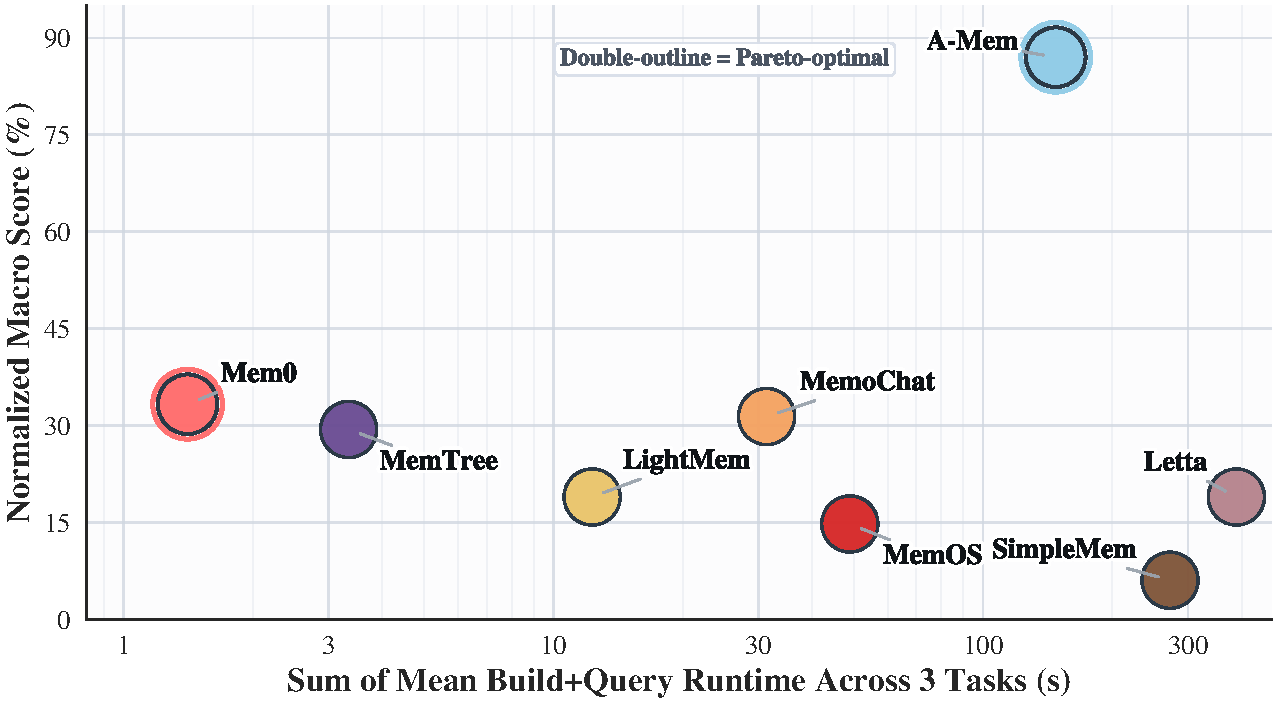
\includegraphics[width=.9\linewidth]{figures/intro_performance.pdf}  
  % \vspace{-.25cm}
  \caption{Performance of Different Agent Memory Methods \zw{(to be refined)}.}
  \label{fig:intro_performance}
  % \vspace{-.68cm}
\end{figure}

\noindent \ding{183} \textit{Agent memory effectively assumes the role of a DBMS.}
The responsibilities of existing agent memory systems closely resemble those of a data management system. They accept write requests when the agent observes new information, process read requests when the agent needs relevant context for reasoning, execute updates when previously stored knowledge changes, manage deletion and compression under limited memory capacity, and maintain consistency in multi-user settings. Together, these functions form a complete data management workload. The key difference is that current agent memory systems are mostly built by the community using machine learning tools, rather than being designed by the database community with DBMS principles and engineering methodologies.

\noindent \ding{184} \textit{Agent memory introduces requirements that are not fully addressed by any existing DBMS.}
Relational databases assume a fixed schema, precise data, and clear query semantics. In contrast, the schema of agent memory evolves as the agent learns, its data often originates from unstructured text and carries uncertainty, and its queries are semantic rather than based on exact matching. Graph databases are effective at representing relationships, but they do not support semantic retrieval well. Vector databases enable semantic retrieval, but they often lack transactions, strict consistency guarantees, and precise relational querying capabilities~\cite{kang2025bigvectorbench}. Temporal databases support version history, but they do not naturally capture knowledge uncertainty or the decay of relevance over time~\cite{rasmussen2025zep}. As a result, no existing DBMS can directly satisfy the full set of requirements for agent memory, leading developers to construct fragmented ``shadow data stacks'' combining multiple heterogeneous stores~\cite{oracle2026agent}. \zxh{-- I don't think it's necessary to mention that relational databases are insufficient for supporting memory. Look for some other points to replace that point instead.}



Despite its importance, during the use of agent memory, there have been numerous complaints and various discoveries. For instance, ... %there are many problems in current agent memory development: (1) the current landscape of agent memory remains highly fragmented; (2) many memories are not agent-native and so have problems when implemented across different agent frameworks and scenarios; (3) current approaches largely overlook system-level optimization opportunities, such as leveraging storage hierarchies, query planning, and execution-aware retrieval. These problems motivate the need for rigorous agent memory evaluation. Current evaluations of agent memory are largely rooted in cognitive science and natural language processing (NLP), focusing primarily on task-level outcomes such as factual recall, long-context understanding, and multi-turn dialogue coherence (e.g., benchmarks like LOCOMO~\cite{maharana2024locomo}, LongMemEval~\cite{wu2024longmemeval}, and MemoryAgentBench~\cite{memoryagentbench2026}). Such evaluations systematically overlook the fundamental nature of agent memory as a complex data management system. At its core, agent memory embodies a database problem involving storage substrates, concurrency control, index maintenance, and cache management. For example, recent empirical studies on the LOCOMO benchmark reveal that while passing the full conversation history in the context window yields high accuracy, it results in unacceptable median latencies of nearly 10 seconds and exorbitant token costs, rendering it unviable for production~\cite{chhikara2025mem0}. Therefore, a principled approach is therefore needed to model and evaluate agent memory as a database-like data management component, along dimensions including data models, update and consistency semantics, retrieval and indexing structures, maintenance and governance, and scalability.

%Despite its importance, there are many problems in current agent memory development: (1) the current landscape of agent memory remains highly fragmented; (2) Many memories are not agent-native and so have problems when implemented across different agent frameworks and scenarios; (3) current approaches largely overlook system-level optimization opportunities, such as leveraging storage hierarchies, query planning, and execution-aware retrieval. These problems motivate the need for agent memory evaluation. Existing benchmarks (e.g., LOCOMO, LongMemEval \zxh{more}) and the evaluation suites embedded in frameworks (e.g., MemGPT, A-Mem \zxh{refs}) primarily focus on retrieval accuracy, reasoning quality, and conversational coherence. While these metrics are essential for assessing the cognitive utility of memory, they largely overlook the fact that agent memory operates as a data management system in practice. Consequently, system-level evaluation remains significantly underexplored. \zxh{add relevant existing evaluations} \zxh{Current evaluations of agent memory are largely rooted in cognitive science and natural language processing (NLP), focusing primarily on task-level outcomes such as factual recall, long-context understanding, and multi-turn dialogue coherence (e.g., benchmarks like LoCoMo and LongMemEval). Such evaluations systematically overlook the fundamental nature of agent memory as a complex data management system. At its core, agent memory embodies a database problem involving storage substrates, concurrency control, index maintenance, and cache management. Therefore, a principled approach is therefore needed to model and evaluate agent memory as a database-like data management component, along dimensions including data models, update and consistency semantics, retrieval and indexing structures, maintenance and governance, and scalability.}

%Key performance indicators from database systems—such as query latency under concurrent workloads, write throughput during sustained agent execution, index maintenance overhead as the memory store evolves, storage amplification across indexing strategies, and consistency guarantees under multi-agent access—are rarely measured in existing benchmarks. This omission creates a critical gap: developers lack principled guidance for selecting and designing memory architectures in production settings, and the fundamental cost–performance trade-offs governing scalability and reliability remain poorly understood.


%Despite this urgency, the current landscape of agent memory remains fundamentally fragmented and under-systematized. First, there lacks clear taxonomy for memory, which can severely hinder choosing the appropriate technology stack and negatively impact the selection and adaptation across different scenarios. \zxh{Second, most existing solutions are not natively integrated with agent execution, treating memory as an external retrieval module rather than a tightly coupled component within the reasoning loop.} Third, current approaches largely overlook system-level optimization opportunities, such as leveraging storage hierarchies, query planning, and execution-aware retrieval, resulting in inefficient and often brittle behavior in realistic workloads. As a result, existing memory solutions remain largely ad hoc, lacking both rigorous design principles and systematic evaluation frameworks. This gap motivates the need for a unified perspective on agent memory, grounded in both qualitative task characteristics and system-level considerations.

% The core memory operations of agents, including storage, indexing, retrieval, consolidation, and forgetting, are fundamentally classic problems in the database literature. \zw{reason $\rightarrow$ why management, illustrate architecture}


% The rise of \llm agents is transforming the underlying models from stateless text generators into stateful systems that require persistent memory to support complex interactions and continual learning.
% In this evolution, agent memory has emerged as a foundational infrastructure that determines whether agents can operate effectively in dynamic environments, enabling long-horizon reasoning, personalization, and continuous adaptation. 



% However, despite the explosive growth of research in this area, the systematic evaluation of agent memory remains fragmented and subject to cognitive biases. Existing memory implementations are scattered across heterogeneous paradigms, such as heuristic rules, vector similarity search, and graph traversal, each exhibiting distinct performance characteristics.

% \noindent \textbf{Memory as Data.}

In this paper, we present the first comprehensive Experimental and Analysis (E\&A) study of agent memory from a database systems perspective.

\noindent \textbf{Contribution.} We propose a Memory-as-Data analytical framework that decomposes agent memory into four core components: representation, storage and indexing, query and routing, and lifecycle management, and systematically maps them to fundamental modules in database systems. Through rigorous benchmarking of mainstream memory paradigms, such as flat vector stores, graph/hybrid indices, and key-value/document stores, on a unified testbed, we go beyond retrieval accuracy to incorporate critical system-level metrics, including latency/throughput, concurrency consistency, index maintenance cost, and space amplification.

Our study aims to uncover the performance trade-offs of different memory architectures under realistic workloads, validate the effectiveness of classical database optimization techniques (e.g., materialized views, adaptive indexing, and transaction control) in agent settings, and establish a new research agenda for the database community centered on agent-oriented data systems.

\noindent $\bullet$ \textbf{Unified Memory-as-Data Framework.}
We present a Memory-as-Data framework that decomposes agent memory into four core components and maps them to fundamental database modules. \zw{architecture}

\noindent $\bullet$ \textbf{Structured Decomposed Taxonomy.}
We establish a clear four-part taxonomy based on representation, storage and indexing, query and routing, and lifecycle management.

\noindent $\bullet$ \textbf{Comprehensive End-to-End Assessment.}
We systematically compare representative memory architectures, including flat vector stores, graph and hybrid indices, and key-value or document-based designs, across single-hop, multi-hop, and long-horizon tasks.

\noindent $\bullet$ \textbf{Fine-grained Component Comparison.}
We study the cost of major memory components, including data ingestion, index maintenance, query routing, and buffer management, and quantify their impact on efficiency and effectiveness.

\noindent $\bullet$ \textbf{Practical Optimization Validation.} \zw{may be removed.}
We implement and evaluate classical database techniques, such as materialized views, adaptive indexing, and transaction control, and show their benefits for latency, resource efficiency, and consistency.

\noindent $\bullet$ \textbf{Forward-looking Research Direction.}
We identify promising directions for the database community, including specialized storage engines, cost-based memory query optimization, and consistency models for multi-agent workloads.


%\zw{concise and short importance illustration, architecture summary, management paradigm}

    % - LLM agents 从实验走向生产部署
    % - Memory 被行业领袖视为下一个关键突破（Sam Altman "infinite perfect memory"）
    % - 各大公司纷纷推出 memory 产品（OpenAI, Microsoft, Google, Anthropic, Oracle）
    % - Memory 已从辅助功能升级为一级架构组件：Component -> System -> Agent?

% agent memory imposes a compound workload that cuts across existing systems abstractions: semantic retrieval plus mutable state, personalization plus governance, long-horizon accumulation plus bounded latency, and multi-agent sharing plus consistency controls. Oracle's recent positioning around a “unified memory core” for agents is actually useful here—not because you should endorse it, but because it shows industry itself is converging on the view that fragmented memory stacks are a real engineering problem.
\fi


% \begin{figure}[!t]
%   % \vspace{-.5cm}
%   \centering
%   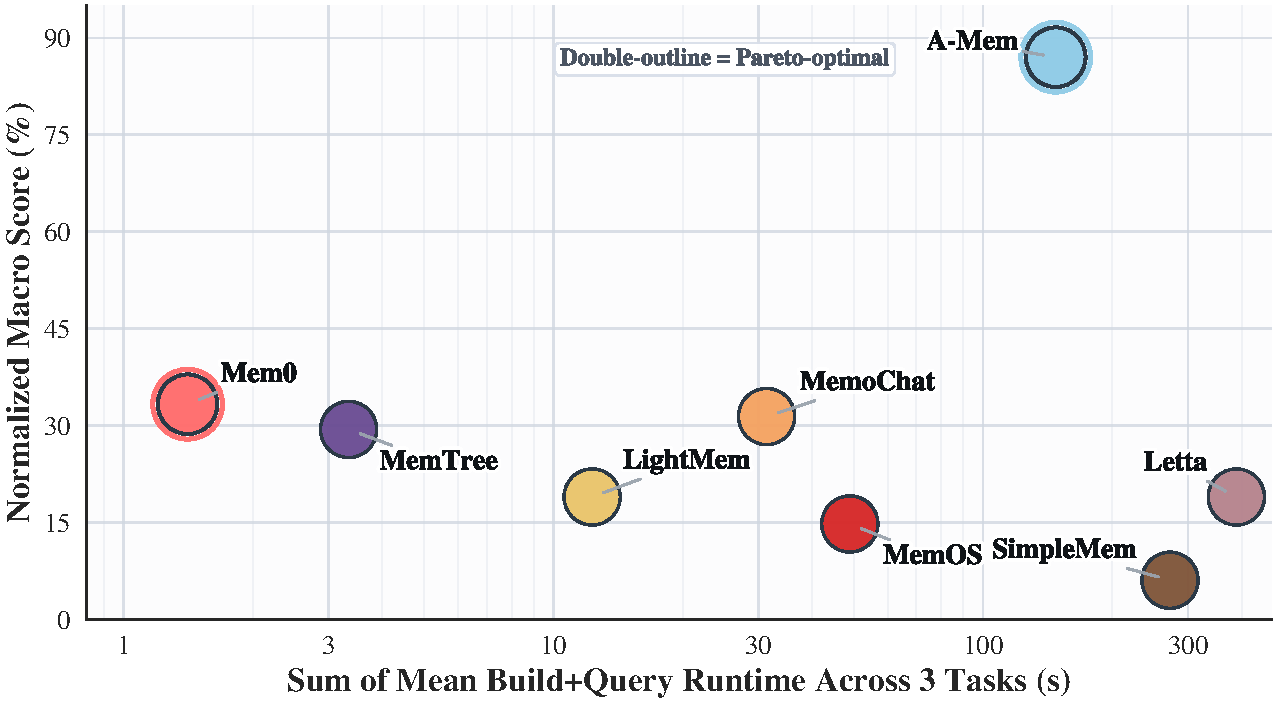
\includegraphics[width=.9\linewidth]{figures/intro_performance.pdf}  
%   % \vspace{-.25cm}
%   \caption{Performance of Different Agent Memory Methods \zw{(to be refined, (a) comparison of agent memory and database system, (b) trending of agent memory systems)}.}
%   \label{fig:intro_performance}
%   % \vspace{-.68cm}
% \end{figure}


%The key difference is that current agent memory systems are mostly built by the AI community using machine learning tools, rather than being designed by the database community with DBMS principles and engineering methodologies. 
% , and multi-turn dialogue coherence

%Compared with traditional data management systems, the current landscape of agent memory remains highly fragmented and lacks systematic evaluation from a data system perspective. 



% , and retrieved through top-$k$ similarity search to augment prompts during inference~\cite{lewis2020retrieval}
% emerged as a fundamental component for supporting agentic workloads and attracted growing attention from both academia~\cite{luo2026data,khan2026rag,liu2026supporting,singh2024personal} and industry~\cite{openai2026agents,microsoft2025copilot,google2025adk}. It manages multi-granularity information, such as historical interactions, domain knowledge, and intermediate execution states~\cite{luo2026data,khan2026rag,liu2026supporting}, and is expected to satisfy increasingly demanding agent requirements, including personalization, long-horizon task completion, and lower inference cost by avoiding repeated context injection. For example, by memorizing the fact that ``Charlie'' is the user's pet, a travel-planning agent can include pet-friendly options (e.g., pet-friendly accommodations) when making the plan of a trip where Charlie can join~\cite{singh2024personal}.

%a later request to \textit{plan a trip where Charlie can join} enables the agent to recover this stored fact and infer an implicit constraint: the itinerary should include pet-friendly options, such as pet-friendly accommodations, even though the user does not explicitly restate this requirement

% At its core, \textit{agent memory is fundamentally a data management problem}: Memory provides historical context to guide reasoning, caches intermediate artifacts produced by tools, and maintains structured state that supports multi-step planning and execution. The responsibilities of existing agent memory systems closely resemble those of a data management system. 

%However, the unique characteristics of agentic workloads bring about new challenges to agent memory, compared with traditional data systems. As shown in \zxh{Figure~\ref{fig:intro} (a)}, 

%in alignment with database's typical components, they accept write requests when the agent observes new information, process read requests when the agent needs relevant context for reasoning, execute updates when previously stored knowledge changes, manage deletion and compression under limited memory capacity, and maintain consistency in multi-user settings. \zxh{discuss in data model, index management, query optimizer / executor} Together, these functions form a complete data management workload. Furthermore, we can observe several significant differences between this system and the underlying design of traditional database systems, \zxh{xxx}.



%, while also supporting dynamic lifecycle governance, such as memory consolidation, temporal decay, and access control.  

%ChatGPT's memory to reference all past conversations (April 2025), a user who had previously mentioned being vegan and living in San Francisco could simply ask "what are some restaurants near me that I'd like," and the agent would autonomously rewrite the query as "good vegan restaurants, San Francisco" by retrieving stored preferences~\cite{openai2024memory}—without such a persistent memory layer, the agent would have no knowledge of the user's dietary restrictions or location, forcing the user to repeat context in every new session.

%As a result, memory is emerging as a \zxh{first-class system problem} rather than an auxiliary feature. 

%Recent studies indicate that agentic workloads, which depend critically on dynamic memory management, are likely to become an important workload class in future data systems. In parallel, major industry platforms are moving memory into the core agent stack.

%Recent academic studies~\cite{luo2026data, khan2026rag, liu2026supporting} highlight that agentic workloads, heavily reliant on dynamic memory management, will soon dominate data systems. Meanwhile, industry leaders are aggressively integrating memory services into their core platforms. For instance, OpenAI has introduced persistent memory mechanisms in its agent stack~\cite{openai2026agents}, and Microsoft (Copilot Memory~\cite{microsoft2025copilot}) and Google (Agent Development Kit~\cite{google2025adk}) are embedding memory services directly into their enterprise and agent development platforms.  %underscoring the strategic necessity of memory in next-generation AI systems.



% while Anthropic has formalized ``context engineering'' and the Model Context Protocol (MCP)~\cite{anthropic2025context, anthropic2024mcp}
